\documentclass{beamer}
\mode<presentation>
{
  \usetheme{ldv}
  \setbeamercovered{transparent}
}

% Uncomment this if you're giving a presentation in german...
%\usepackage[ngerman]{babel}

% ...and rename this to "Folie"
\newcommand{\slidenomenclature}{Slide}


\usepackage[utf8]{inputenc}
\usepackage{amsmath,amssymb,amsfonts}
\usepackage{times}
\usepackage{graphicx}
\usepackage{fancyvrb}
\usepackage{array}
\usepackage{colortbl}
\usepackage{tabularx}

% Uncomment me when you need to insert code
\usepackage{color}
\usepackage{listings}
% End Code

% Uncomment me when you need video or sound
\usepackage{multimedia}
\usepackage{hyperref}
% End video

% Header
\newcommand{\zwischentitel}{ARL Project}
\newcommand{\leitthema}{Alperen Gündogan, Rachid Ellouze, Uzair Akbar}
% End Header

% Titlepage
\title{ARL Project}
\author{Alperen Gündogan, Rachid Ellouze, Uzair Akbar}
\newcommand{\presdatum}{May 2019}
\institute
{
  Lehrstuhl für Datenverarbeitung\\
}
\subtitle{Sometimes we also need a subtitle}
% End Titlepage


% Slides
\begin{document}

% 1. Slide: Titlepage
\begin{frame}
	\titlepage
\end{frame}

% 2. Slide: TOC
\begin{frame}
   \frametitle{Table of contents}
   \tableofcontents[subsectionstyle=hide]
\end{frame} 

% Further Slides
\section{Titles} 
\begin{frame}
   \frametitle{Title} 
   Each frame should have a title.
\end{frame}



\subsection{Subsection no.1.1  }
\begin{frame} 
   Without title something is missing. 
\end{frame}



\section{Lists} 
\subsection{Lists I}
\begin{frame}
   \frametitle{Unnumbered Lists}
   \begin{itemize}
      \item Introduction to  \LaTeX  
      \item Second bullet point 
      \item And a third one
      \item The last one
   \end{itemize} 
\end{frame}



\begin{frame}\frametitle{Lists with Pause}
   \begin{itemize}
      \item Introduction to  \LaTeX \pause 
      \item Second bullet point \pause 
      \item And a third one \pause 
      \item The last one
   \end{itemize} 
\end{frame}



\subsection{Lists II}
\begin{frame}
   \frametitle{Numbered Lists}
   \begin{enumerate}
      \item Introduction to  \LaTeX  
      \item Second bullet point 
      \item And a third one
      \item The last one
   \end{enumerate}
\end{frame}



\begin{frame}
   \frametitle{Numbered Lists with Pause}
   \begin{enumerate}
      \item Introduction to  \LaTeX \pause 
      \item Second bullet point \pause 
      \item And a third one \pause 
      \item The last one
   \end{enumerate}
\end{frame}



\section{Tables} 
\subsection{Tables}
\begin{frame}
   \frametitle{Tables}
   \begin{tabular}{|c|c|c|}
      \hline
      \textbf{Title} & \textbf{Title} & \textbf{Title} \\
      \hline
      First column & Second column &  \LaTeX  \\
      \hline
      Second row & \LaTeX & Last column \\
      \hline
   \end{tabular}
\end{frame}



\section{Blocks \& Math}
\subsection{Blocks}
\begin{frame}
   \frametitle{Blocks}

   \begin{block}{This is a simple block}
      It should contain some text.
   \end{block}

   \begin{exampleblock}{Example Block}
      This may be an example.
   \end{exampleblock}


   \begin{alertblock}{Warning}
      The violent color indicates that this block may alert of something.
   \end{alertblock}
\end{frame}



\subsection{Math} 
\begin{frame}
   \frametitle{Math Expressions are a Breeze with \LaTeX \ldots}

   \begin{equation}
      p(\mathbf{x}_{k}|\mathbf{Z}_{k}) = \frac{p(\mathbf{z}_{k}|\mathbf{x     }_{k})p(\mathbf{x}_{k}|\mathbf{Z}_{k-1})}{\int \! p(\mathbf{z}_{k}|\mathbf{     x}_{k})p(\mathbf{x}_{k}|\mathbf{Z}_{k-1})\,d\mathbf{x}_{k}}
   \end{equation}

   \begin{equation}
      w_{k}^{i} \sim w_{k-1}^{i}\frac{p(\mathbf{z}_{k}|\mathbf{x}_{k}^{i})p(\mathbf{x}_{k}^{i}|\mathbf{x}_{k-1}^{i})}{q(\mathbf{x}_{k}^{i}|\mathbf{x}_{k-1}^{i},\mathbf{z}_{k})}
   \end{equation}

   \ldots and Bayes filtering is great!

\end{frame}



\section{Colors}
\begin{frame}
   \frametitle{An Overview of TUM's Colors}
   \tiny{Color blue sRGB 100\%: 0-101-189} \\
   \colorbox{tumcolor-blue}{}{}  \\
   \vspace{0.5cm}
   \tiny{Color green sRGB 100\%: 162-173-0} \\
   \colorbox{tumcolor-green}{}{} \\
   \vspace{0.5cm}
   \tiny{Color light grey sRGB 100\%: 218-215-203} \\
   \colorbox{tumcolor-lightgrey}{}{} \\
   \vspace{0.5cm}
   \tiny{Color orange sRGB 100\%: 227-114-34} \\
   \colorbox{tumcolor-orange}{}{} \\
   \vspace{0.5cm}
\end{frame}



\section{Multimedia}
\subsection{Split Screen}
\begin{frame}
   \frametitle{Splitting Screen}
   \begin{columns}

      \begin{column}{5cm}
         \begin{itemize}
            \item Here
            \item is some
            \item text
         \end{itemize}
      \end{column}

      \begin{column}{5cm}
         \begin{tabular}{|c|c|}
            \hline
            \textbf{On the} & \textbf{other side} \\
            \hline
            there may &  be a table \\
            \hline
            or even &  a picture as  \\
            \hline
            shown on the &  next frame  \\
            \hline
         \end{tabular}
      \end{column}

   \end{columns}
\end{frame}



\subsection{Pictures} 
\begin{frame}
   \frametitle{Pictures in Latex Beamer Class}
   \begin{figure}
      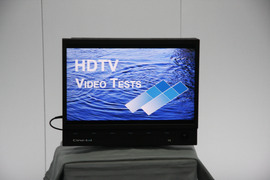
\includegraphics[scale=2.0]{images/video} 
      \caption{This is a picture!}
   \end{figure}
\end{frame}



\subsection{Pictures which Need More Space} 
\begin{frame}[plain]
   \frametitle{Plain, or a Way to Get More Space}
   \begin{figure}
      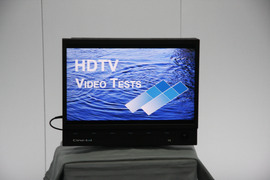
\includegraphics[scale=3.0]{images/video} 
      \caption{Picture again.}
   \end{figure}
\end{frame}



\subsection{Code Listings} 
% The [fragile] is important for listings!
\begin{frame}[fragile]
   \frametitle{Don't Ever Bore the Audience with Code Listings}
   \lstset{language=C, basicstyle=\small \ttfamily, showspaces=false, showtabs=false, tab= , keywordstyle=\bfseries, showstringspaces=false, framexleftmargin=5mm, frame=single, numbers=left, numberstyle=\tiny, stepnumber=1, numbersep=5pt, texcl=true}
   \begin{lstlisting}[caption={Especially when they are erroneous},frame=tlrb]
#include <stdio.h>

int main(void)
{
  printf("Hallo Welt\n");
  while(1);
  return 0;
}
   \end{lstlisting}
\end{frame}

% End Slides

\end{document}
